\documentclass[10pt,conference]{IEEEtran}
%\usepackage[bottom=0.62in]{geometry}
\usepackage[latin1]{inputenc}
\usepackage[T1]{fontenc}
\usepackage{fancyvrb}
\usepackage{times}
\usepackage{amsmath,amssymb}
\usepackage{url}
\usepackage{graphicx}
\usepackage{caption, subcaption}
\usepackage{framed}
\usepackage[usenames,dvipsnames]{xcolor}
\usepackage{listings}
\usepackage{xspace}
\usepackage{multirow}
\usepackage{enumitem}
 \usepackage{booktabs}


% Set the default teletype font to txtt.
\renewcommand{\ttdefault}{txtt}

% Set the default style for listsings.
\lstset{language=C,
        basicstyle=\ttfamily\small,
        keywordstyle=\bfseries,
        stringstyle=,
        xleftmargin=1em,
        showstringspaces=false,
        commentstyle=\rmfamily\itshape,
        columns=flexible,
        keepspaces=true,
        texcl=true,
        literate={\-}{}{0\discretionary{-}{}{}}
}

% Inline code.
\newcommand{\code}[1]{\lstinline @#1@}

% Define an environment for C++ programs.
\lstnewenvironment{codeblock}{\lstset{language=C}}{}



\renewcommand{\baselinestretch}{1.01}
 
\newcommand{\secref}[1]{$\S$~\ref{#1}}

\setlength{\parskip}{0pt}   % No separatation between paragraphs
\setlength{\FrameSep}{0pt}
\setlist{noitemsep}         % No spearation between list bullets

\usepackage[inline]{trackchanges}
\addeditor{alex}
\addeditor{prithviraj}
\addeditor{muxi}


\newcommand{\alex}[1]{\add[as]{#1}}
\newcommand{\alexn}[1]{\notee[as]{#1}}
\newcommand\alexr[1]{}%  {\remove[as]{#1}}
\newcommand\alexa[2]{\annote[as]{#2}{#1}}

\newcommand{\prithviraj}[1]{\add[prithviraj]{#1}}
\newcommand{\prithvirajn}[1]{\notee[prithviraj]{#1}}

\newcommand{\muxi}[1]{\add[muxi]{#1}}
\newcommand{\muxin}[1]{\notee[muxi]{#1}}

\newcommand{\red}[1]{\textcolor{red}{ #1}}

\newcommand{\aetherflow}{{\AE}therFlow\xspace}
\newcommand{\crossflow}{CrossFlow\xspace}

\hyphenation{of-soft-switch}

%\def\blfootnote{\xdef\@thefnmark{}\@footnotetext}


%\newcommand\blfootnote[1]{%
%  \begingroup
%  \renewcommand\thefootnote{}\footnote{#1}%
%  \addtocounter{footnote}{-1}%
%  \endgroup
%}



%\newcommand\blfootnote[1]{%
%  \begingroup
%  \renewcommand\thefootnote{}\footnote{#1}%
%  \addtocounter{footnote}{-1}%
%  \endgroup
%}


\begin{document}
	
	\addtolength{\topmargin}{-0.61\baselineskip}

\title{Enabling Dynamic Reconfigurability of SDRs Using SDN Principles}
%\title{\crossflow: A Cross-layer Architecture for SDR Using SDN Principles}

\author{
  \IEEEauthorblockN{Prithviraj Shome\IEEEauthorrefmark{1}, Jalil Modares\IEEEauthorrefmark{2}, Nicholas Mastronarde\IEEEauthorrefmark{2}, and Alex Sprintson\IEEEauthorrefmark{1}} 
  \IEEEauthorblockA{\IEEEauthorrefmark{1}Department of Electrical and Computer Engineering, Texas A\&M University} 
%        College Station, Texas, USA \\
%       \{prithvirajhi,mxyan, spalex\}@tamu.edu}
%  \and
%  \IEEEauthorblockN{Sayedjalil Modares Najafabad, Nicholas Mastronarde}
  \IEEEauthorblockA{\IEEEauthorrefmark{2}Department of Electrical Engineering, University at Buffalo} 
%       Buffalo, New York, USA \\
%       \{sayedjal,nmastron\}@buffalo.edu}
}

\maketitle 


%\blfootnote{This  material is based upon work supported by the National Science Foundation under Grants No. 1422655, 1423322, by the AFOSR under contract \mbox{No. FA9550-13-1-0008,} and by the Air Force Research Laboratory under Grant \mbox{No. FA8750-14-1-0073.}\\
%}

\begin{abstract}
Dynamic reconfiguration and network programmability are active research areas. State of the art solutions use the Software Defined Networking (SDN) paradigm to provide basic data plane abstractions and programming interfaces for control and management of these abstractions. This approach provides the benefit of control and data plane separation, but it is mainly limited to wired networks. Currently, SDN technologies do not provide appropriate abstractions to support constantly evolving wireless protocols. On the other hand, the Software Defined Radio (SDR) paradigm enables complex signal processing functionality to be implemented efficiently in software, instead of on specialized hardware. However, SDR does not cater to the demand for adaptive radio network management with respect to changing channel conditions and policies. 
%Current approaches focus upon specific protocol implementations and do not provide a generic and principled framework for developing network applications. 
To address this, we present \crossflow, a principled approach for application development in radio networks. \crossflow defines several fundamental radio port abstractions and an interface to manipulate them. The framework provides a flexible and modular cross-layer architecture using the principles of SDR and a mechanism for centralized control using the principles of SDN. The main feature of the \crossflow architecture is that it provides a protocol independent framework for application development in wireless radio networks. We validate our design using proof-of-concept applications, namely, adaptive modulation, frequency hopping, and cognitive radio. Our results indicate that our framework is efficient, flexible, and can be used for a variety of applications.
\end{abstract}


%\blfootnote{This  material is based upon work supported by the National Science Foundation under Grants No. 1422655, 1423322 and by the AFOSR under contract  \mbox{No. FA9550-13-1-0008.}\\
%This paper appeared in the CoolSDN Workshop of ICNP 2015.
%}

\section{Introduction}
\label{sec:intro}
With ever-changing wireless standards and protocols, there has been a conscious shift towards a programmatic approach for designing and implementing wireless radios. This has led to a tremendous interest in Software Defined Radios (SDR). SDR is a powerful concept in which filters, amplifiers, modulators and other complex signal processing blocks are realized in software, instead of on specialized hardware. As the task of signal processing is handed over to software, it is possible to use general purpose hardware, connected to an RF front end, to create powerful and highly flexible radios.

While the SDR paradigm has revolutionized the design of wireless radios, it does not provide an efficient method to control a network of SDRs. Since SDRs can be reconfigured to provide a wide variety of radio functionalities, it would be highly desirable to have a consistent interface to expose the SDR's functional modules to the application developer. As modules can be added, removed or changed any time, such an interface framework must be able to adapt to these changes, report events to the application, and allow control of various constituent modules while hiding their complexity from the application developer. This level of abstraction is necessary because, as the network grows and becomes more heterogeneous, it is impossible for the application developer to keep track of low-level details. Here, by the notion of heterogeneous networks, we take into consideration a network containing both wired and wireless devices. Hence the architecture should enable network control, meet requirements of users and at the same time abstract away the details of the implementation.

In order to provide abstractions taking into account the above considerations, we use the concept of Software Defined Networking (SDN). SDN defines abstractions that represent data plane components along with the interface to control and manage these abstractions. As a result, these primitives (including asynchronous callback function event reporting) enable an application developer to obtain a logically centralized view of the network. The application developer can then dynamically adjust rules to reflect changing network conditions and requirements.

In this paper, we aim to integrate SDR and SDN to provide a principled approach for developing a consistent interface to manage underlying abstractions of SDRs. We build upon the abstract model presented in our previous paper \cite{crossflow}, where we described a monolithic architecture for \emph{wireless radio port} abstraction. In the current paper, we go beyond that and broaden the design space to provide a modular design, which is in line with the design principle of SDR.
%As the design does not make any assumption about the protocols to be supported, the framework remains independent of network protocols and helps in building a true cross layered architecture platform. 
This also enables an integration of both wired and wireless networks which can be managed in a programmatic manner, thereby enabling development of key applications catering to a heterogeneous network. We call our platform \crossflow. Some network applications that we envision can leverage \crossflow include, but are not limited to, the following:
\begin{itemize}
\item \emph{Physical layer adaptation} including:
\begin{enumerate}
	\item \emph{frequency hopping} to resist narrowband interference and prevent unauthorized interception; 
	\item \emph{transmission power control} to maintain a target link quality while reducing interference to other users and/or extending battery life;
	\item \emph{adaptive modulation and coding} to trade-off throughput and communication reliability and adapt to channel conditions (e.g., pathloss and interference).
\end{enumerate}

%(i)  %In Section~\ref{sec:evaluation}, we present an implementation of frequency hopping and adaptive modulation using the \crossflow framework.

\item \emph{Quality of service (QoS) provisioning} to provide QoS policies according to profiles implemented through medium access control, throttling, admission control, scheduling, and error control techniques (e.g., ARQ and FEC). This allows both coarse-grained and fine-grained QoS policies to be defined in the network.

\item \emph{Adaptive routing} to allow a  \crossflow controller, with its global view of the network, to dynamically switch between existing proactive and reactive routing protocols, and novel software-defined routing protocols, depending on the network conditions and the application constraints.

% \item \emph{Adaptive routing} to allow a distributed \crossflow controller, with its global view of the network, to dynamically switch between reactive and proactive routing protocols depending on the network conditions and the application constraints.

\item \emph{Self healing network} to allow the \crossflow controller to deploy fault management applications based upon self-healing mechanisms.

\item \emph{Cross-layer control} to allow joint optimization of parameters, algorithms, and protocols at all layers of the protocol stack.
\end{itemize}

We use the generalized model of SDN introduced in \cite{Casey:14} as a template for defining the abstractions and their features discussed above. We also build upon the concept of \emph{wireless radio ports} as discussed in \cite{aetherflow}. This abstraction is composed of a number of smaller abstractions, one for each processing block, so that fine-grained control of the processing capabilities of a radio device is provided to application developers without exposing its intricate details. This enables manipulation of critical physical, data link (including the medium access control sublayer), and network layer properties through various well defined interfaces. Thus using the architecture of \crossflow, we can build applications across all layers of the network stack.

For validation purposes, we use the popular GNU Radio~\cite{gnuradio}, which provides a modular  open-source Digital Signal Processing (DSP) software framework for SDRs. The modules of GNU Radio are written in C++ and provide a mechanism to connect and manage data between them. A Python wrapper ties these blocks together to implement applications. We host GNU Radio on a Universal Software Radio Peripheral (USRP) N210 device from Ettus Research and also run CPqd SoftSwitch software~\cite{ofsoftswitch13} as a separate module. CPqd SoftSwitch serves as a switch agent interacting between the SDN controller and GNU Radio modules. This is done through message extensions which we will discuss in subsequent sections. We also develop three proof-of-concept applications to validate our design principles: \emph{frequency hopping}, \emph{adaptive modulation}, and \emph{cognitive radio}.

Our contributions can be summarized as follows.

\begin{itemize}
\item We propose a framework that provides a uniform and consistent view of SDRs, so that a network of SDRs can be managed in an efficient manner.

\item We extend the SDN model with message extensions to provide support for wireless radio interfaces.

\item We provide sample applications using the framework for validation.
\end{itemize}

The rest of the paper is organized as follows. In Section~\ref{sec:related} we review the related work done in this area. Section~\ref{sec:architecture} describes the \crossflow architecture with its SDN extensions. Section~\ref{sec:evaluation} describes a proof-of-concept implementation of three applications using our framework. Section~\ref{sec:conclusion} concludes the paper and discusses future work.

\section{Related Work}
\label{sec:related}

The idea of providing a flexible MAC was implemented by various vendors in the form of \textit{soft-MAC}\cite{softmac}, where most of the time critical operations like synchronization, transmission and reception operations were deployed in hardware, while the other non-critical operations like admission control and rate control were performed in software. However this technique does not provide full control of MAC layer properties to the programmer. Some solutions like the Software Defined Radio framework provided by \cite{gnuradio} try to provide flexibity but it suffers from throughput loss. Other Software Defined Radio initiatives like \cite{sora} try to provide a hardware-like throughput, but suffers from inflexibity due to its complex architecture and requires significant expertise for operation. 

\cite{macproc} provides a high degree of programmability of MAC layer as it represents each MAC protocol as a finite state machine and provides a set of interfaces to manipulate the state of the machine. In fact, we use the paper's interfaces to define our own MAC abstraction layer. The paper \cite{maclet} extends \cite{macproc} by allowing the installation of a \textit{on-the-fly} full MAC protocol logic, rather than a set of parameter settings. The main difference between these works and our work is that we focus on providing an abstract layer for the interfaces exposed by the NIC vendor in a consistent manner, so as to avoid ad-hoc approaches. This allows applications to be developed in a much easier way, and provides a clean separation between application logic and implementation. The previous papers mainly focus on mechanisms to provide these interfaces, which is orthogonal to our work. The exisiting approaches use details which are too low level and need sophisticated handling by the application to implement an event based asynchronous programming model.  

\section{\crossflow Architecture and Design}
\label{sec:architecture}

In this section, we describe the architecture and design of \pmac. In Section~\ref{sec:mac}, we introduce the proposed MAC layer abstraction. Then, in Section~\ref{sec:topology}, we describe the topology in which the \pmac operates and in Section~\ref{sec:messages}, we describe how we extend the OpenFlow protocol to accommodate \pmac messages.


\begin{figure}[t]
  \centering
  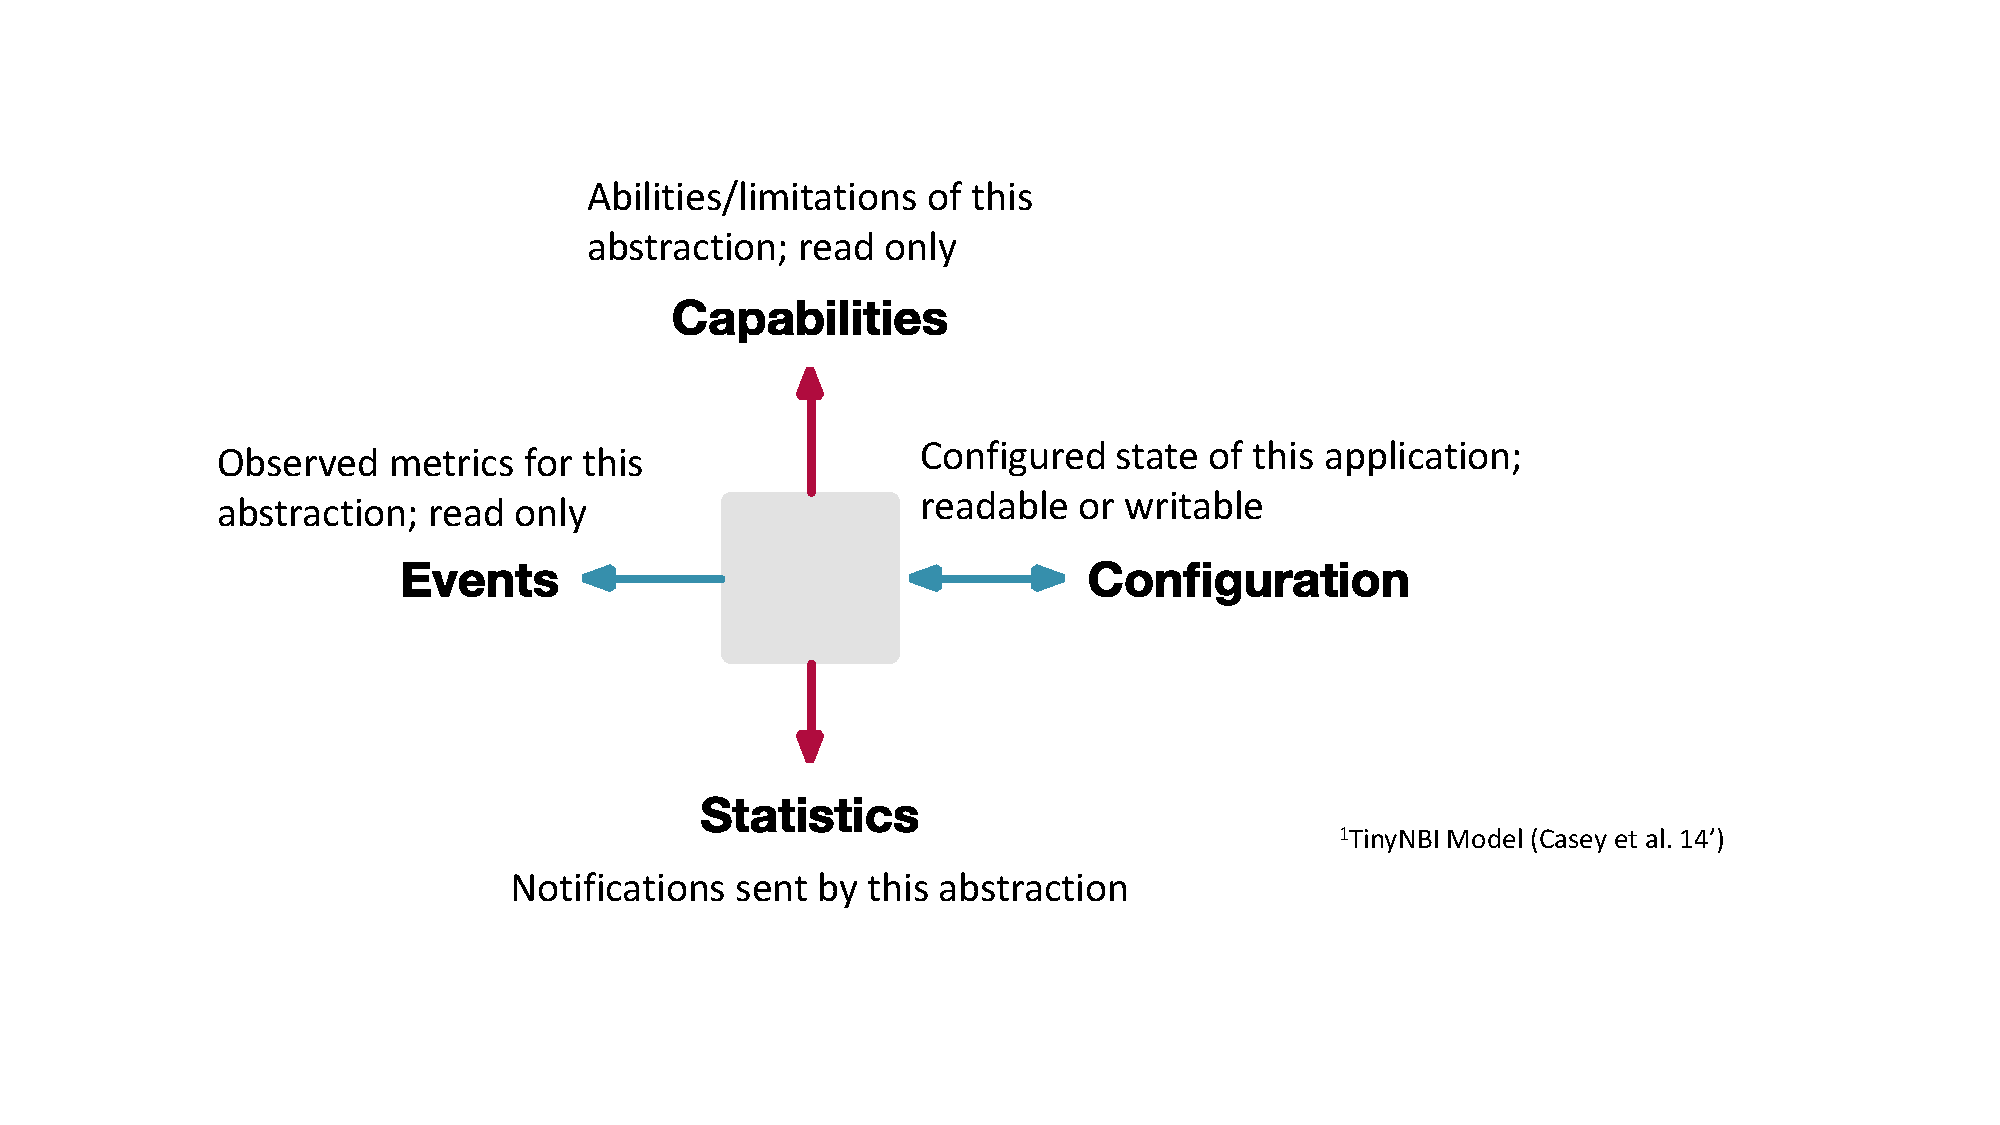
\includegraphics[width=0.6\textwidth]{figures/abstract.pdf}
  \caption{Interfaces exposed by an abstract entity}
  \label{fig:abstract}
\end{figure}

\begin{figure}[t]
  \centering
  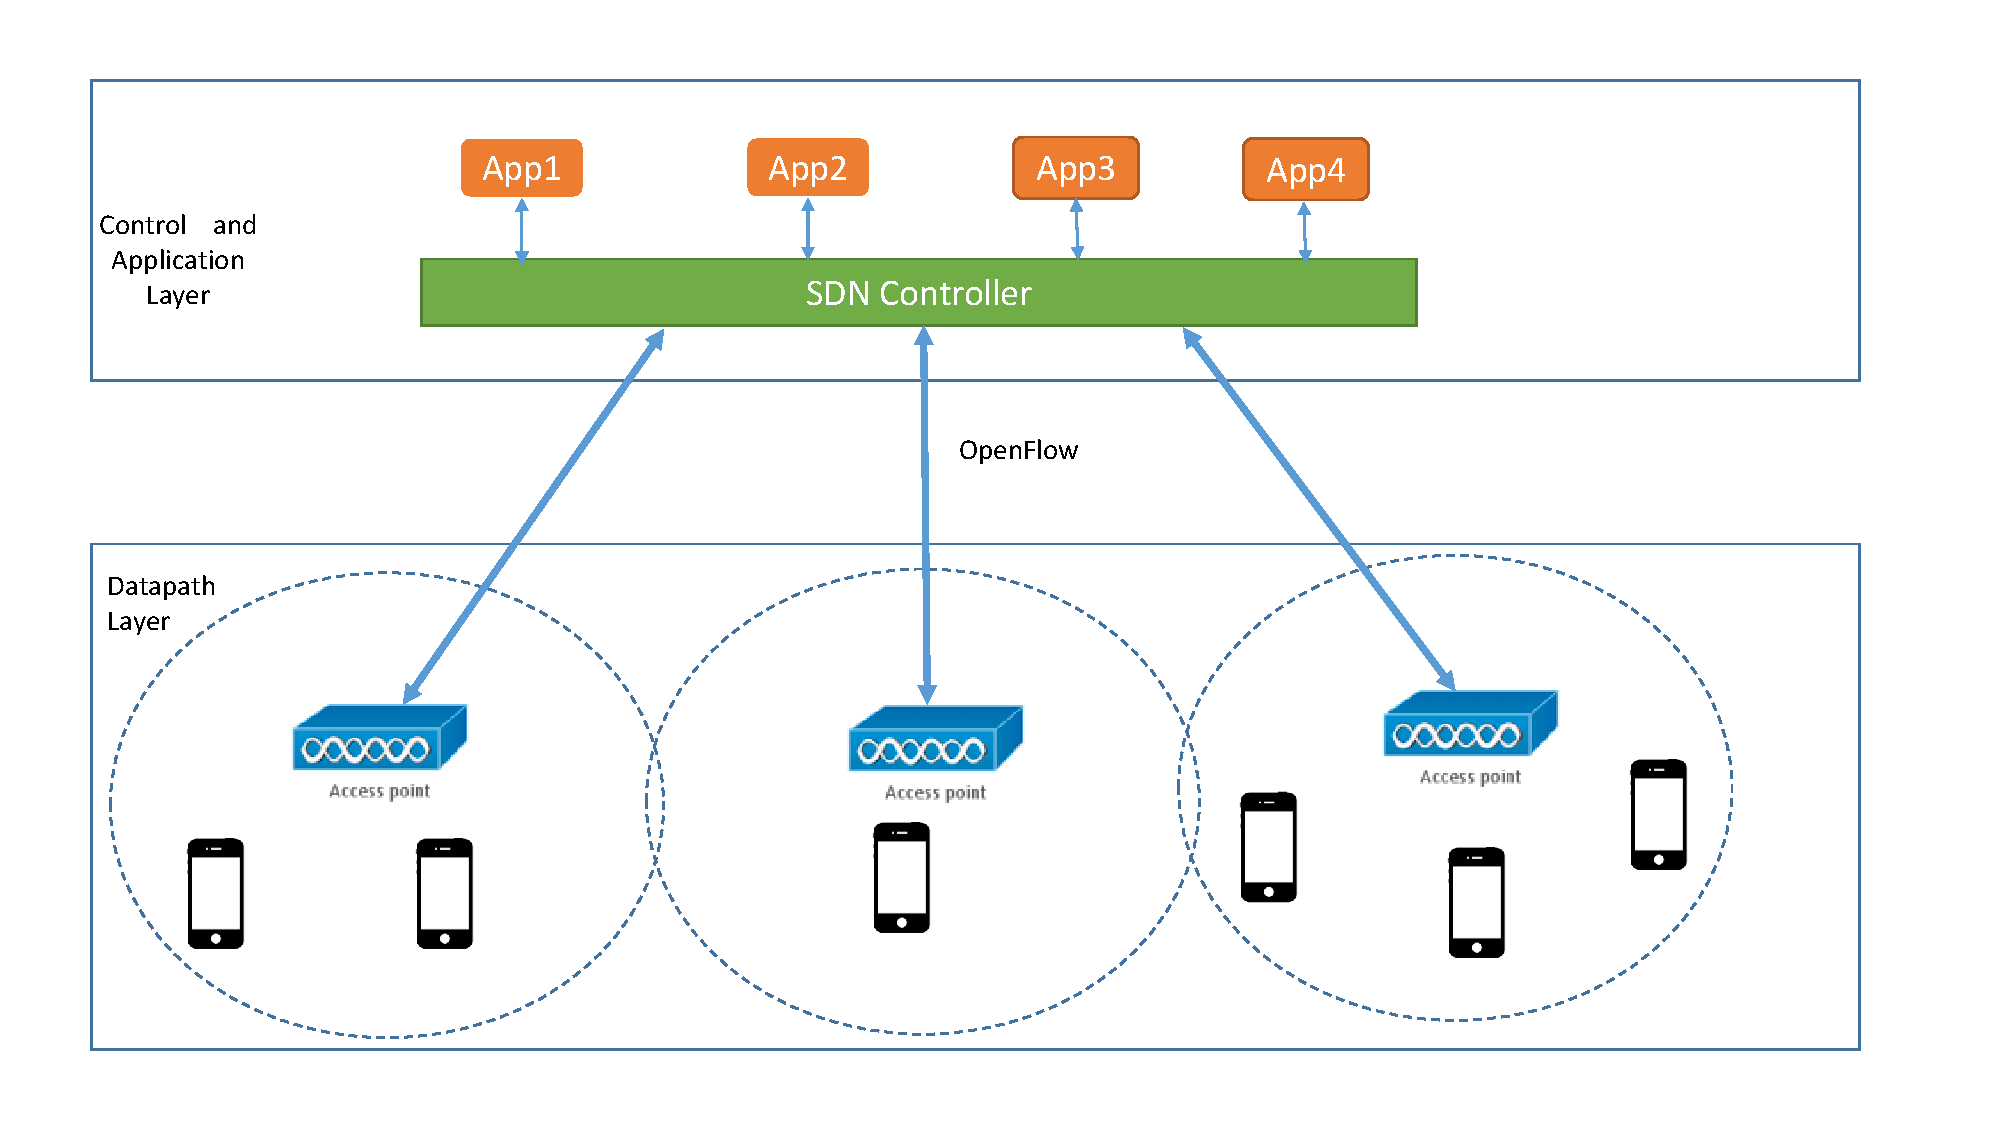
\includegraphics[width=0.6\textwidth]{figures/infrastructure.pdf}
  \caption{Infrastructure diagram of \pmac}
  \label{fig:infrastructure}
\end{figure}

\subsection{MAC Layer Abstraction}
\label{sec:mac}
We use the TinyNBI model described in \cite{Casey:14}, where each abstract component exposes these four types of interfaces: configuration, capability, statistics and events as shown in Figure~\ref{fig:abstract}. As mentioned in Section~\ref{sec:intro}, we take the interface definitions from \cite{macproc} and categorize them in the following manner:

\begin{itemize}
\item \textbf{Capabilities}: The interface allows the SDN controller to query the capabilities of MAC layer such as:
    (i) MAC protocol being used;
    (ii) Maximum frame length and
    (ii) Transmit power  
\item \textbf{Configuration}: The interface allows the SDN controller to configure the properties of MAC layer such as:
    (i) Setting backoff interval;
    (ii) Updating congestion window;
    (ii) Changing MAC protocol; and
    (iv) Setting timer value  
\item \textbf{Statistics}: The interface allows the SDN controller to query the statistics of MAC layer such as:
    (i) Queue length;
    (ii) Cuurent backoff interval and
    (ii) Number of frames received  
\item \textbf{Configuration}: The interface allows the SDN controller to register for events of MAC layer such as:
    (i) Collissions;
    (ii) Channel up/down;
    (ii) Queue overflow; and
    (iv) Timer expiry  
\end{itemize}

\begin{figure}[t]
  \centering
  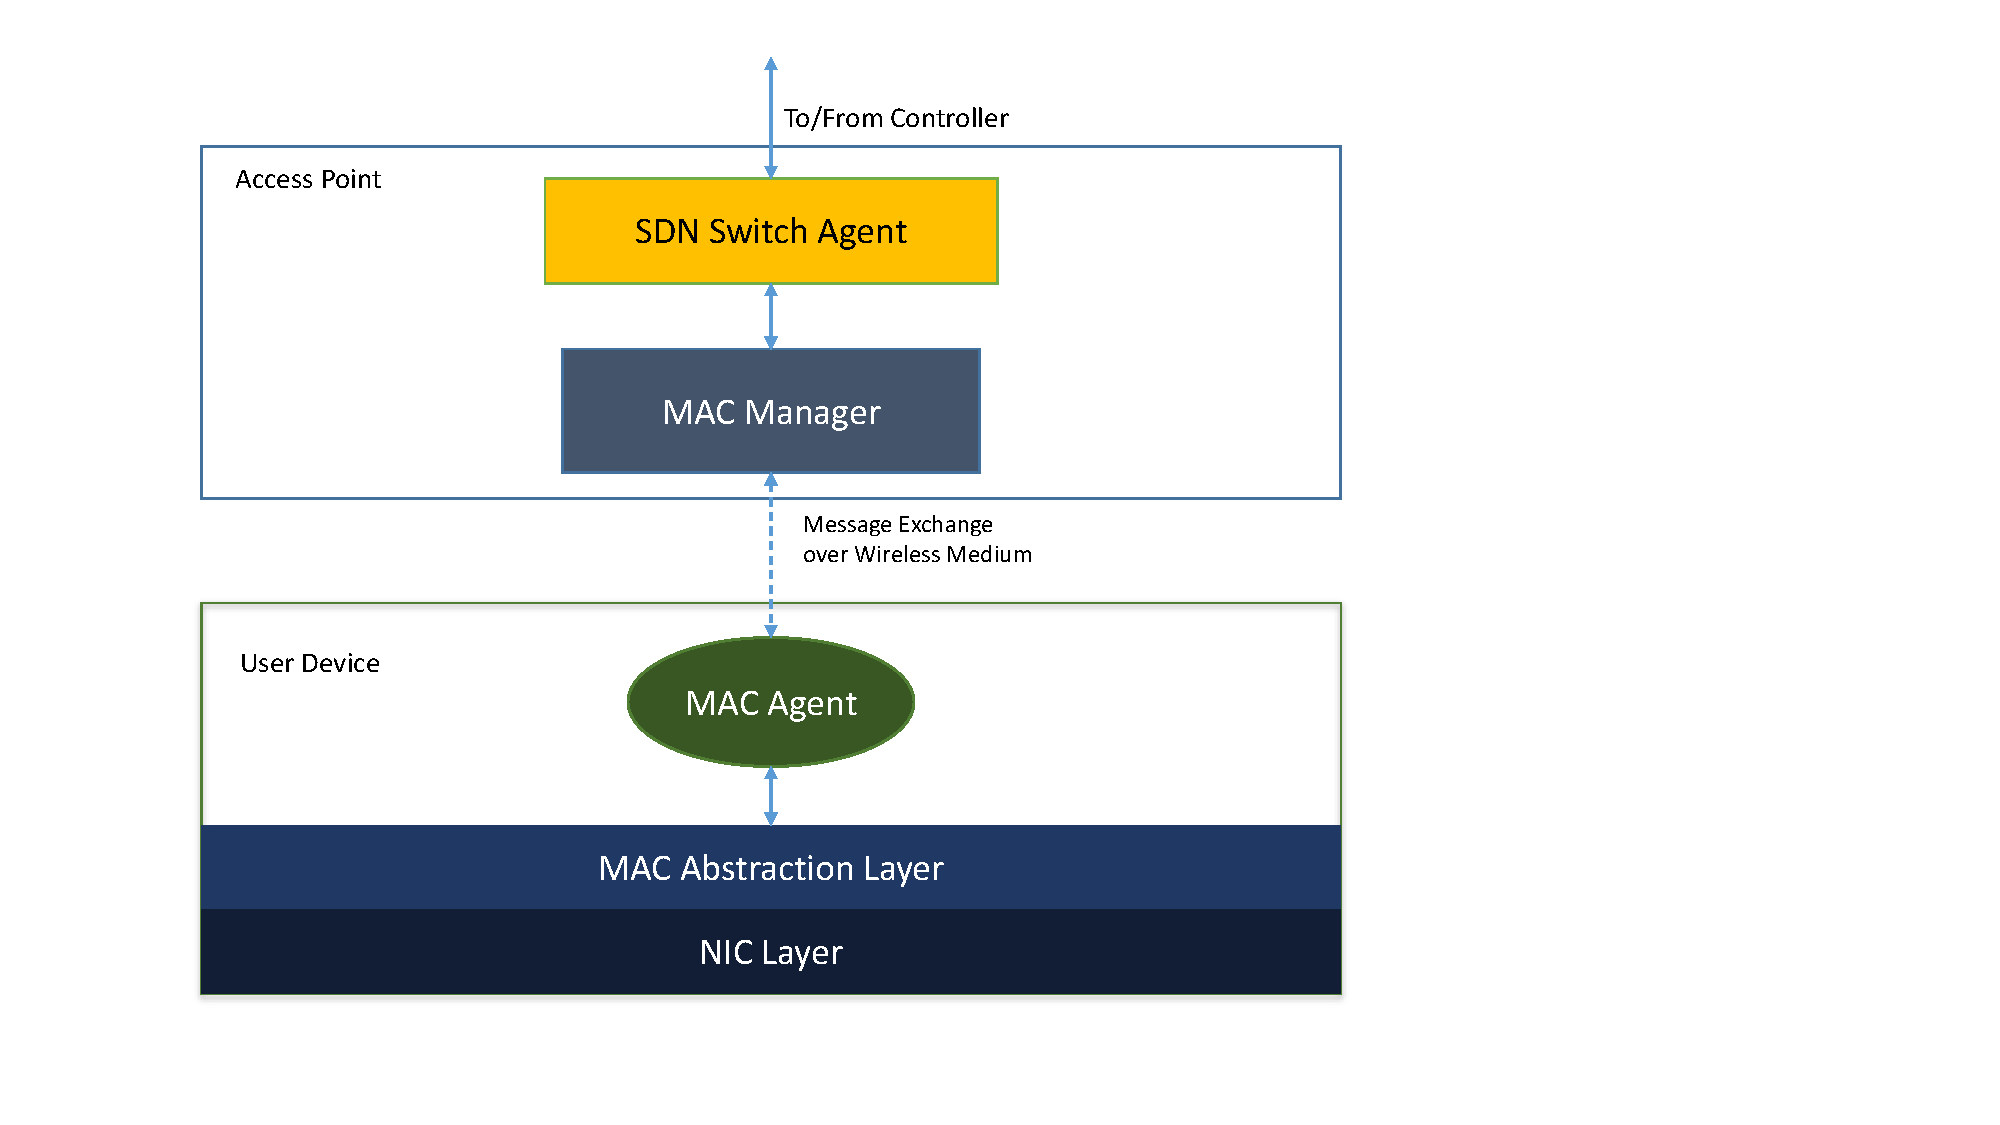
\includegraphics[width=0.6\textwidth]{figures/communication.pdf}
  \caption{MAC Manager (AP), MAC Agent and MAC abstraction layer(User devices) interaction}
  \label{fig:topology}
\end{figure}

\subsection{\pmac Topology}
\label{sec:topology}
In this paper, we consider the \pmac framework in a wireless network which operates in infrastructure mode as shown in Figure~\ref{fig:infrastructure}. The wireless clients are connected to the Access Points (AP), which are in turn, connected to a SDN controller. Each wireless client is composed of a MAC abstraction layer and a MAC agent running on top which is responsible for a MAC manager running in the AP. The MAC abstraction layer, on the other hand, is responsible for exposing the interface types as mentioned above. In a typical deployment scenario, the controller will send request to the AP, which is received by the MAC manager. The MAC manager then sends this requests to all the MAC agents running in the devices. This information can be piggybacked in beacon responses between devices and AP. On the response side, the MAC agents collect the information from the MAC abstraction layer and sends the information to MAC manager in AP through beacon requests. These responses are collected from all the devices associated with the AP, and an event report is sent to the controller. An illustrative diagram of this operation is shown in Figure~\ref{fig:topology}. 

\begin{figure}[t]
  \centering
  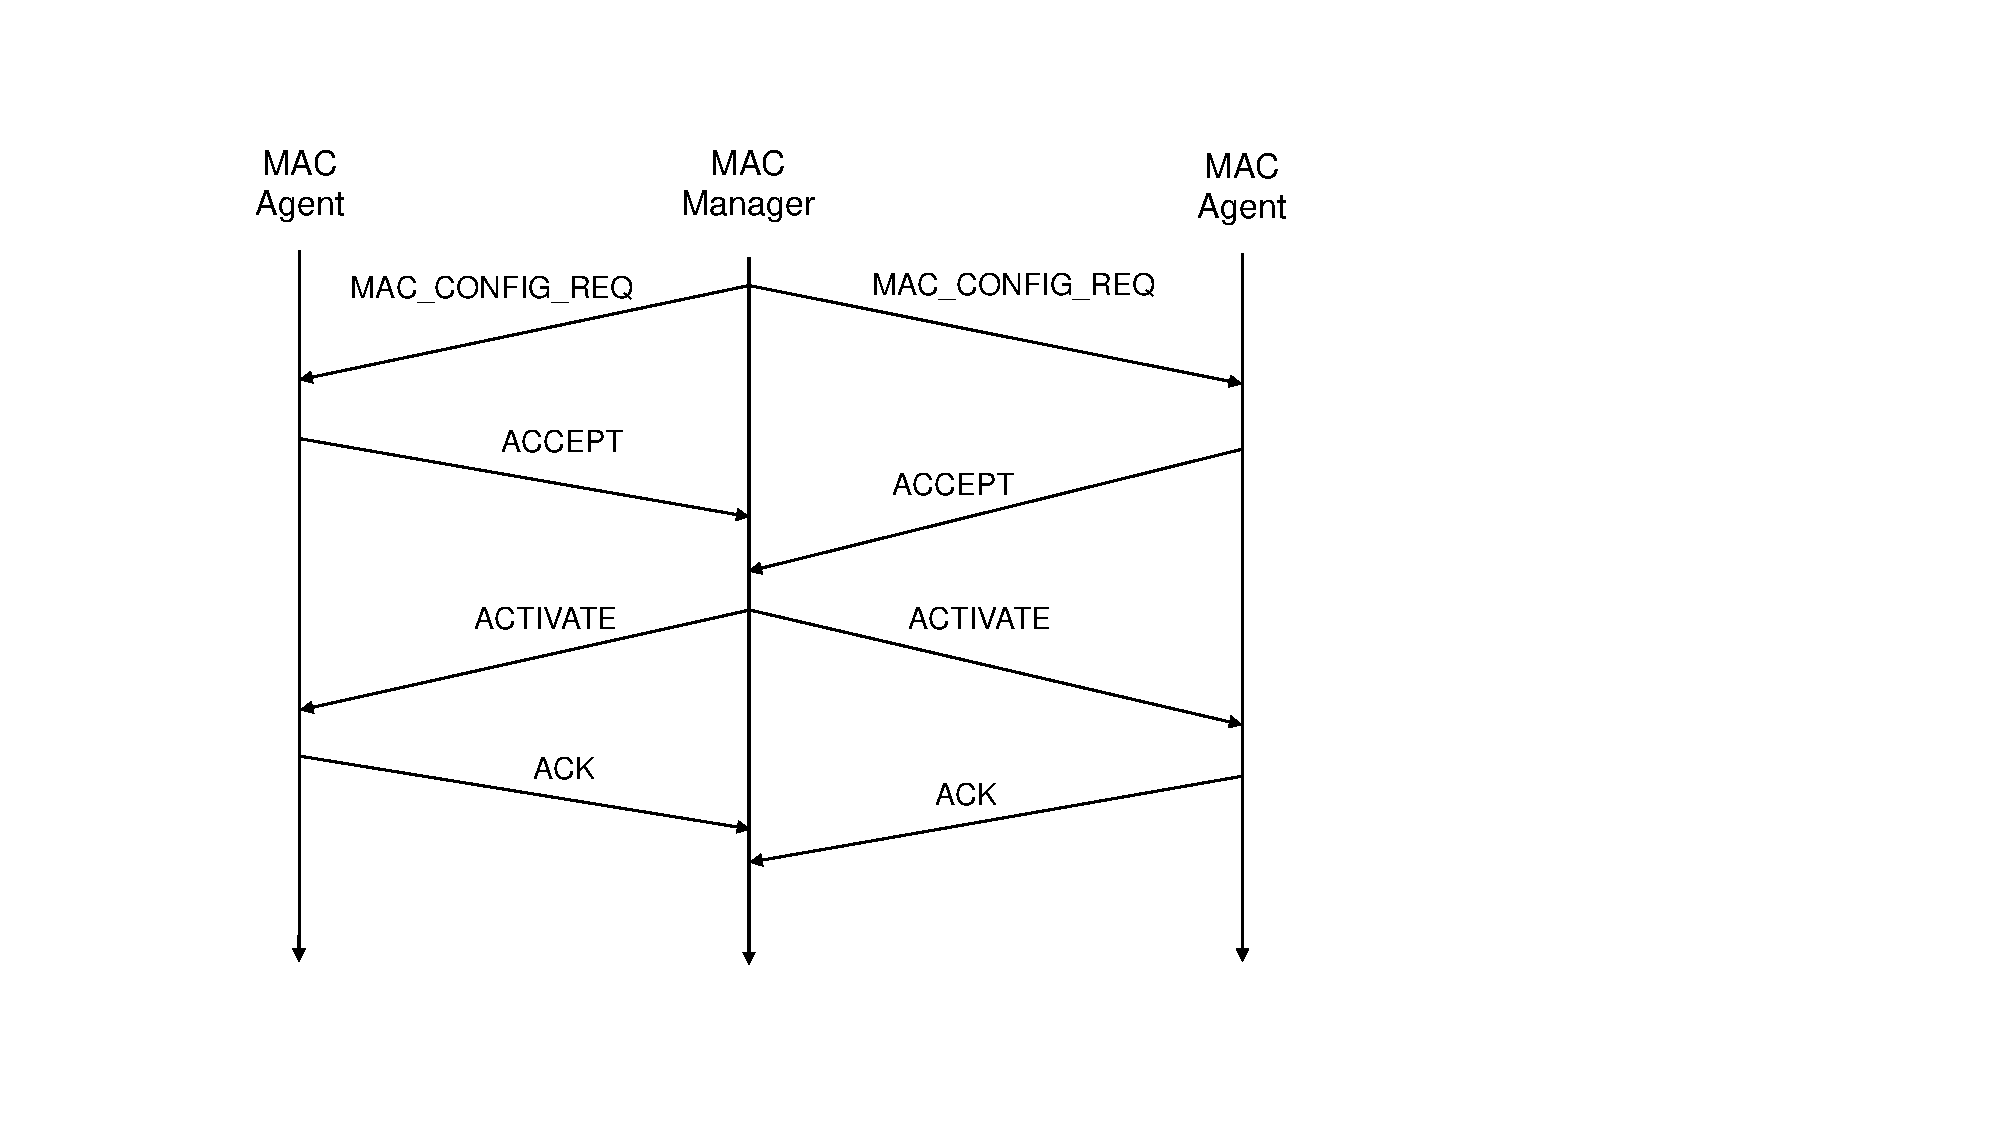
\includegraphics[width=0.6\textwidth]{figures/protocol.pdf}
  \caption{4-way handshake model between MAC Manager and MAC Agent for configuration messages in \pmac}
  \label{fig:protocol_feature}
\end{figure}

In order to support configuration messages, the \pmac framework needs to consider the synchronization issue which may arise due to inconsistencies  while applying the configuration. We developed a 4-way handshake protocol between the MAC manager and MAC agents so that configuration messages are applied in a reliable manner. As shown in Figure~\ref{fig:protocol_feature}, in the first step, the MAC Manager sends a \texttt{MAC-CONFIG-REQ} to all the MAC agents. Upon receiving this request, the agents communicate with the MAC abstraction layer to load the configuration and send  \texttt{ACCEPT} messages to the MAC Manager. Upon receiving all the \texttt{ACCEPT} messages, the MAC Manager sends \texttt{ACTIVATE} message to the agents to activate the configuration. Upon successful application of configuration, the agents send an \texttt{ACK} response and the MAC Manager informs the controller about the change of configuration. If any failure happens, similar process is used to rollback the configuration and a report is sent to the controller 

\subsection{Message Extensions}
\label{sec:messages}
  		  
\pmac uses SDN design principles to configure the MAC layer of devices thorough APs. As OpenFlow protocol does not natively support wireless MAC layer functionality, we extend the OpenFlow protocol to include such messages. For implementation purposes, we can use Experimenter fields of OpenFlow protocol which is used to define vendor specific information. We envision the following OpenFlow message extensions in \pmac:
\begin{itemize}
\item Capabilities message request - Request for the capability of MAC layer of devices like MAC protocl being used, frame length etc
\item Configuration message request - Request for modification of parameters like MAC protocol, timer value etc.
\item Statistics message request - Request for statistics such as queue length, current backoff interval etc.
\item Event message response - Response for events like collissions, timer expiry etc.
\end {itemize}

\section{Proof-of-Concept Implementation}
\label{sec:evaluation}

\subsection{Implementation}

In this section, we describe our implementation of the system using the GloMoSim simulation software. Since it is proof-of-concept, we simplify the system. The controller is an application on the same machine running GloMoSim, and so does not require Openflow for communication. We also assume a simple event model wherein we assume that the controller has information about the state of the network and accordingly decides on an action. We add two modules in GloMoSim to receive commands from the controller and to reconfigure or change the MAC protocols of the nodes. We open a socket between the controller and one of the modules in GloMoSim for sending the commands. The other module performs the actual switching of MAC protocols of all the nodes in the simulation. It is also responsible for performing the 4-way handshake between the MAC Manager and the MAC Agents. The abstractions of SDN switch agent, MAC Manager and MAC Agent are merged into these two modules in our implementation. 

\begin{figure}[t]
  \centering
  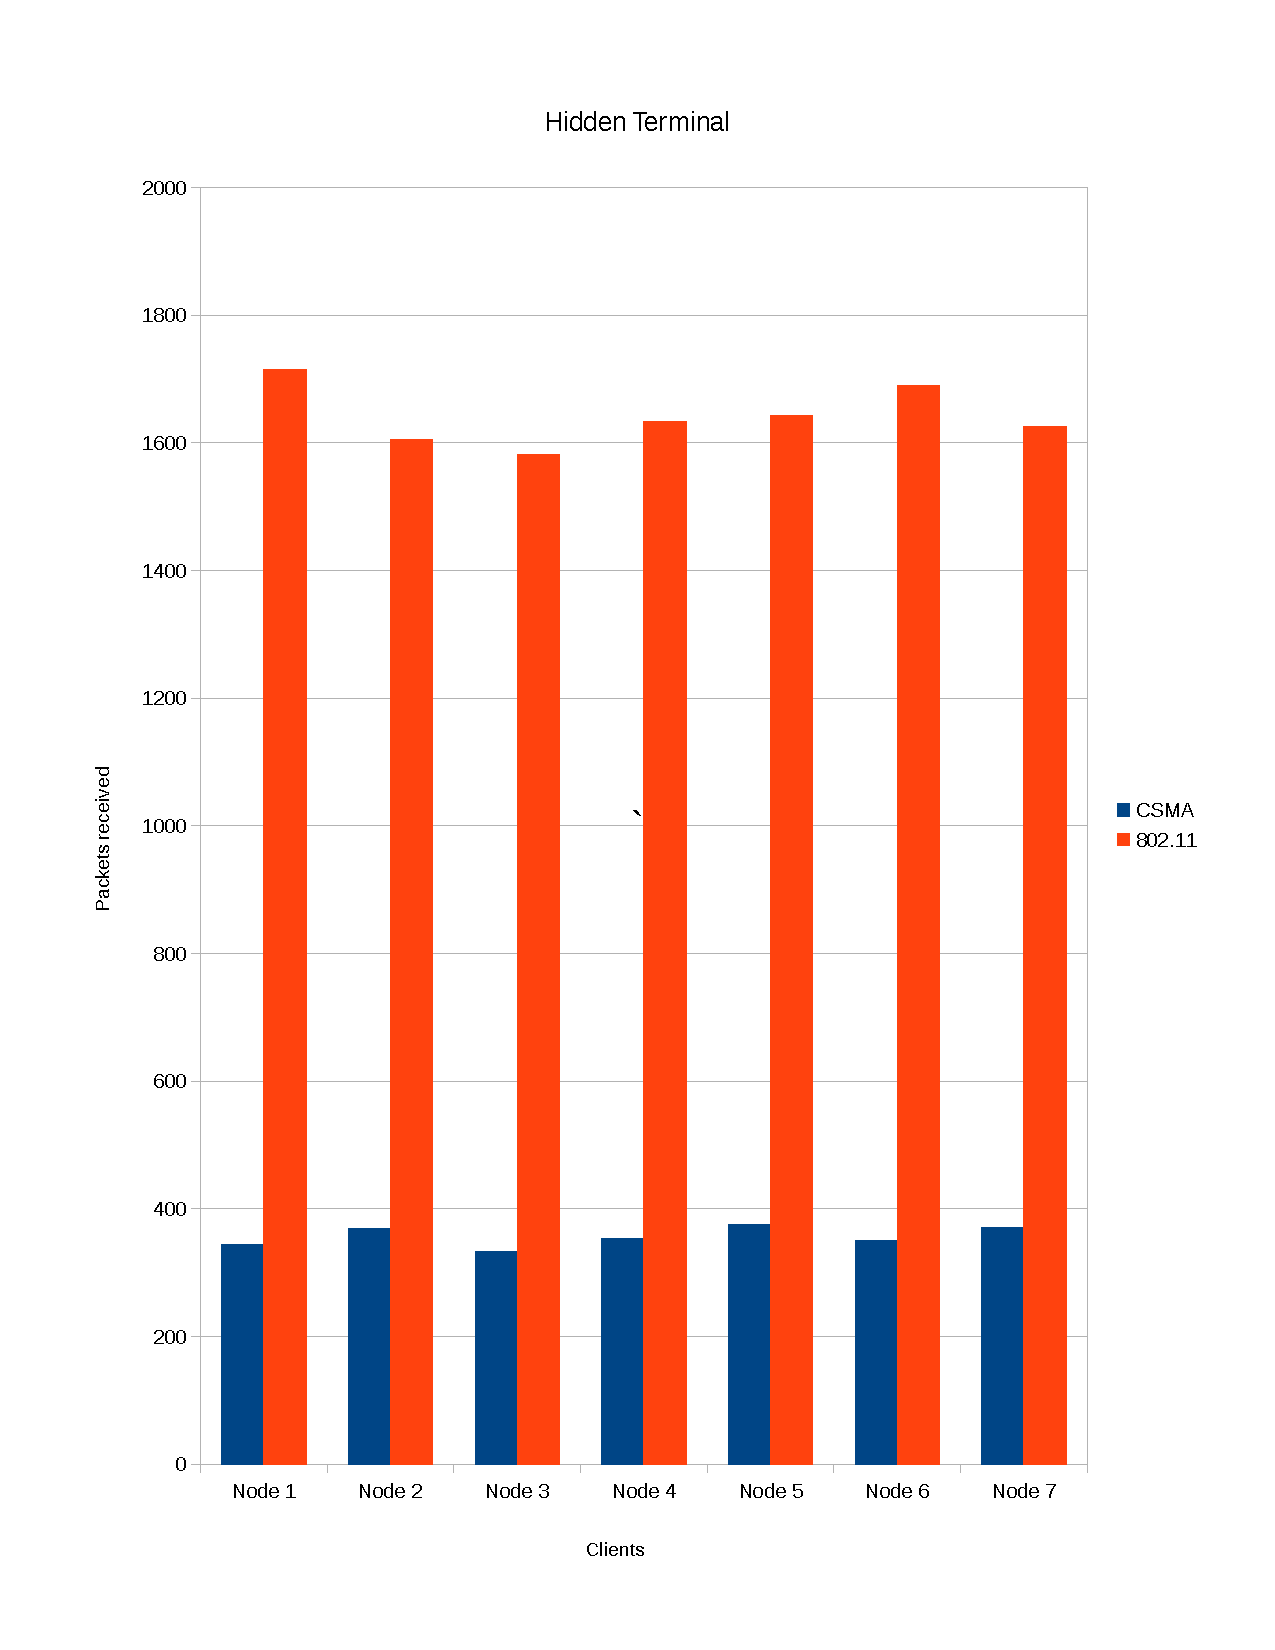
\includegraphics[width=0.35\textwidth, scale=0.5]{figures/hidden_recvPkts.pdf}
  \caption{Change in the number of received packets as the MAC protocol is changed from CSMA to 802.11}
  \label{fig:setup}
\end{figure}

\begin{figure}[t]
  \centering
  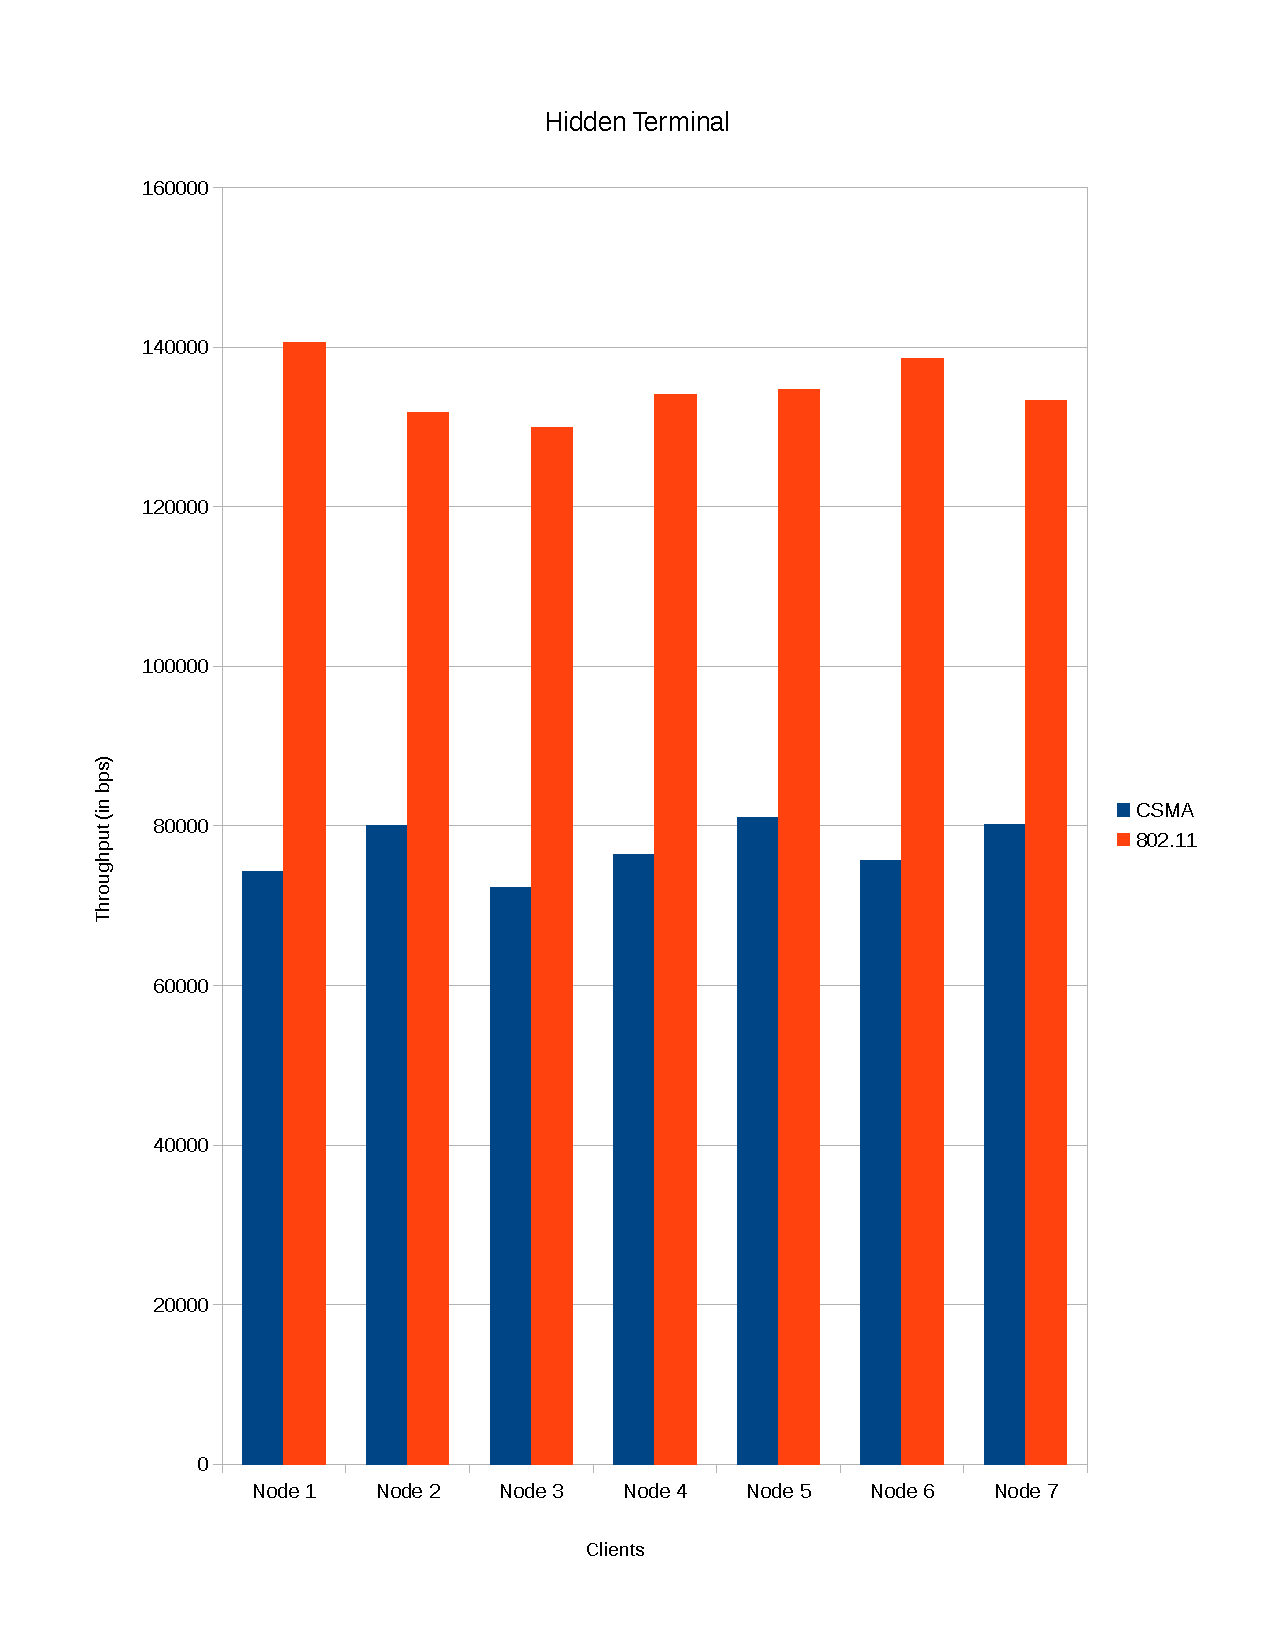
\includegraphics[width=0.35\textwidth, scale=0.5]{figures/hidden_thrput.pdf}
  \caption{Change in throughput of the nodes as the MAC protocol is changed from CSMA to 802.11}
  \label{fig:overhead}
\end{figure}

\begin{figure}[t]
  \centering
  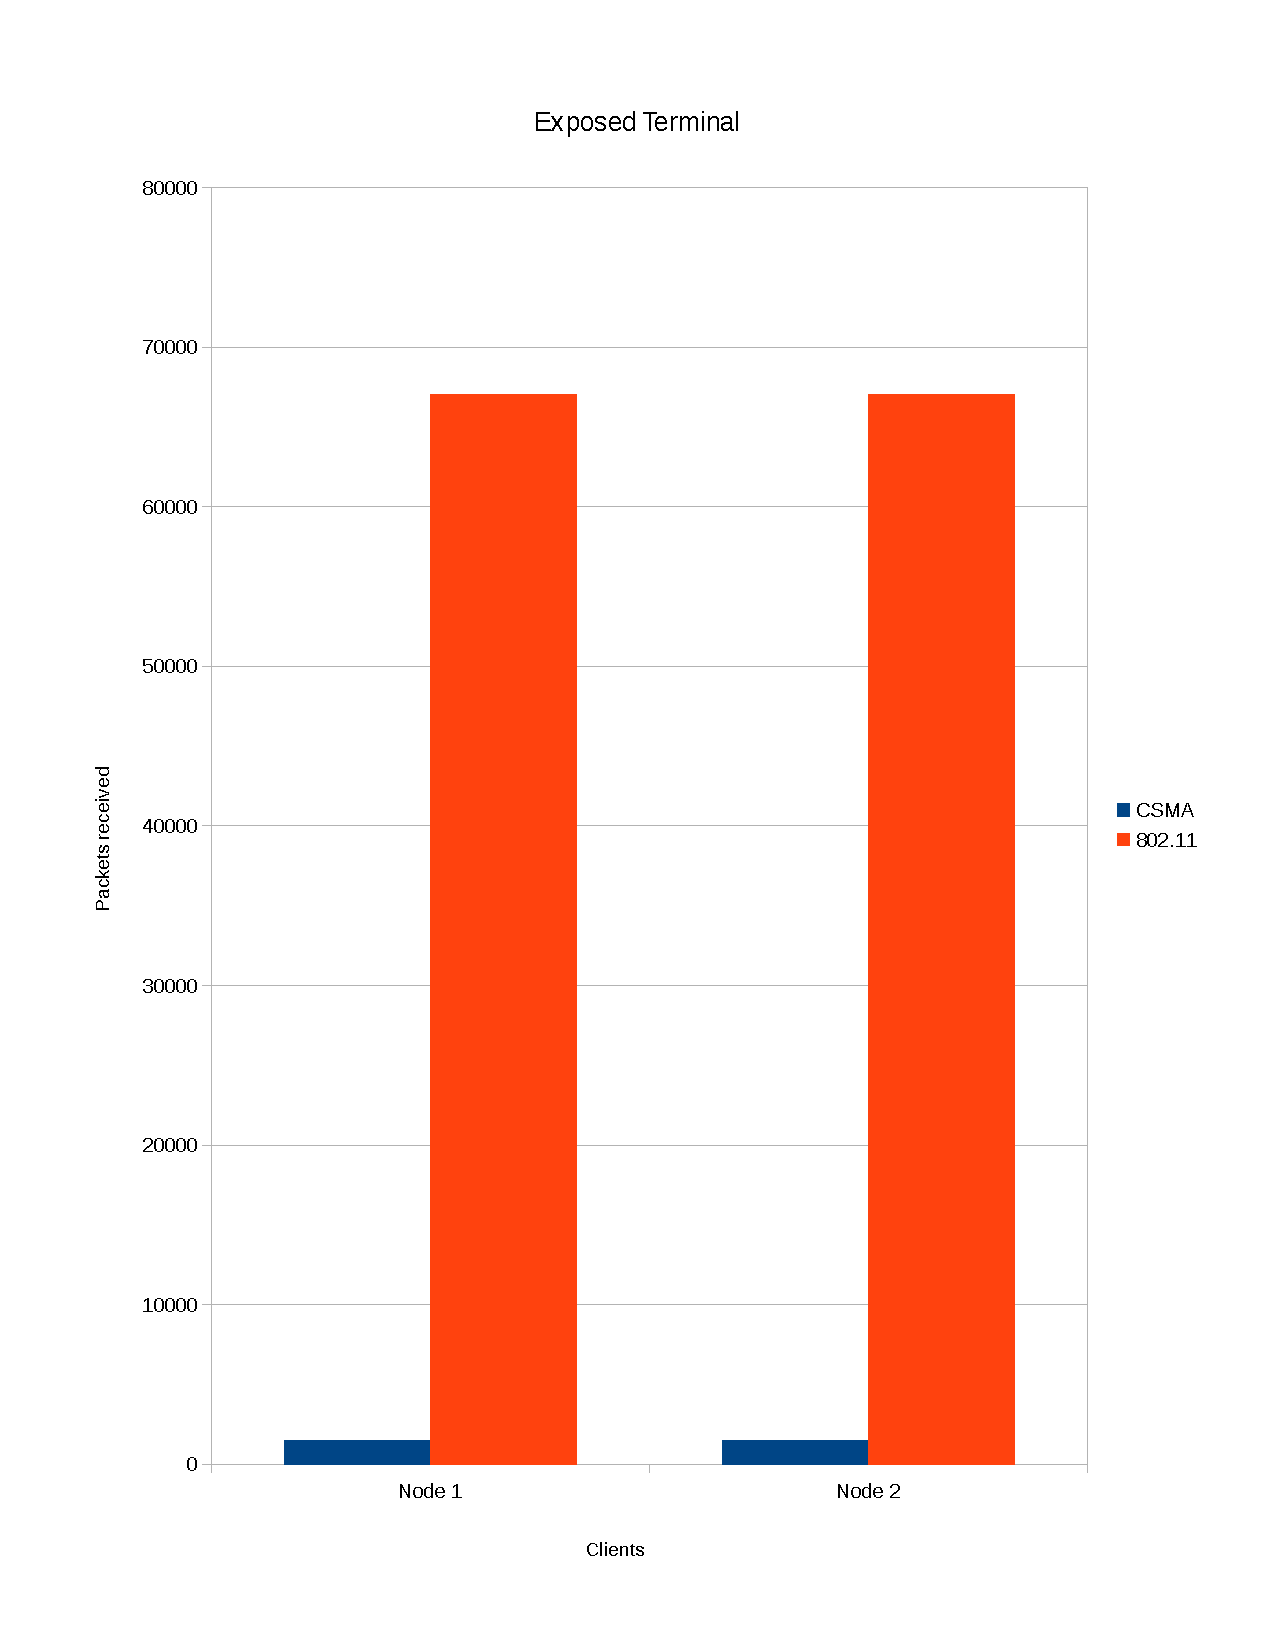
\includegraphics[width=0.35\textwidth, scale=0.5]{figures/exposed_recvPkts.pdf}
  \caption{Change in the number of received packets when the MAC is changed from CSMA to 802.11}
  \label{fig:setup}
\end{figure}

\begin{figure}[t]
  \centering
  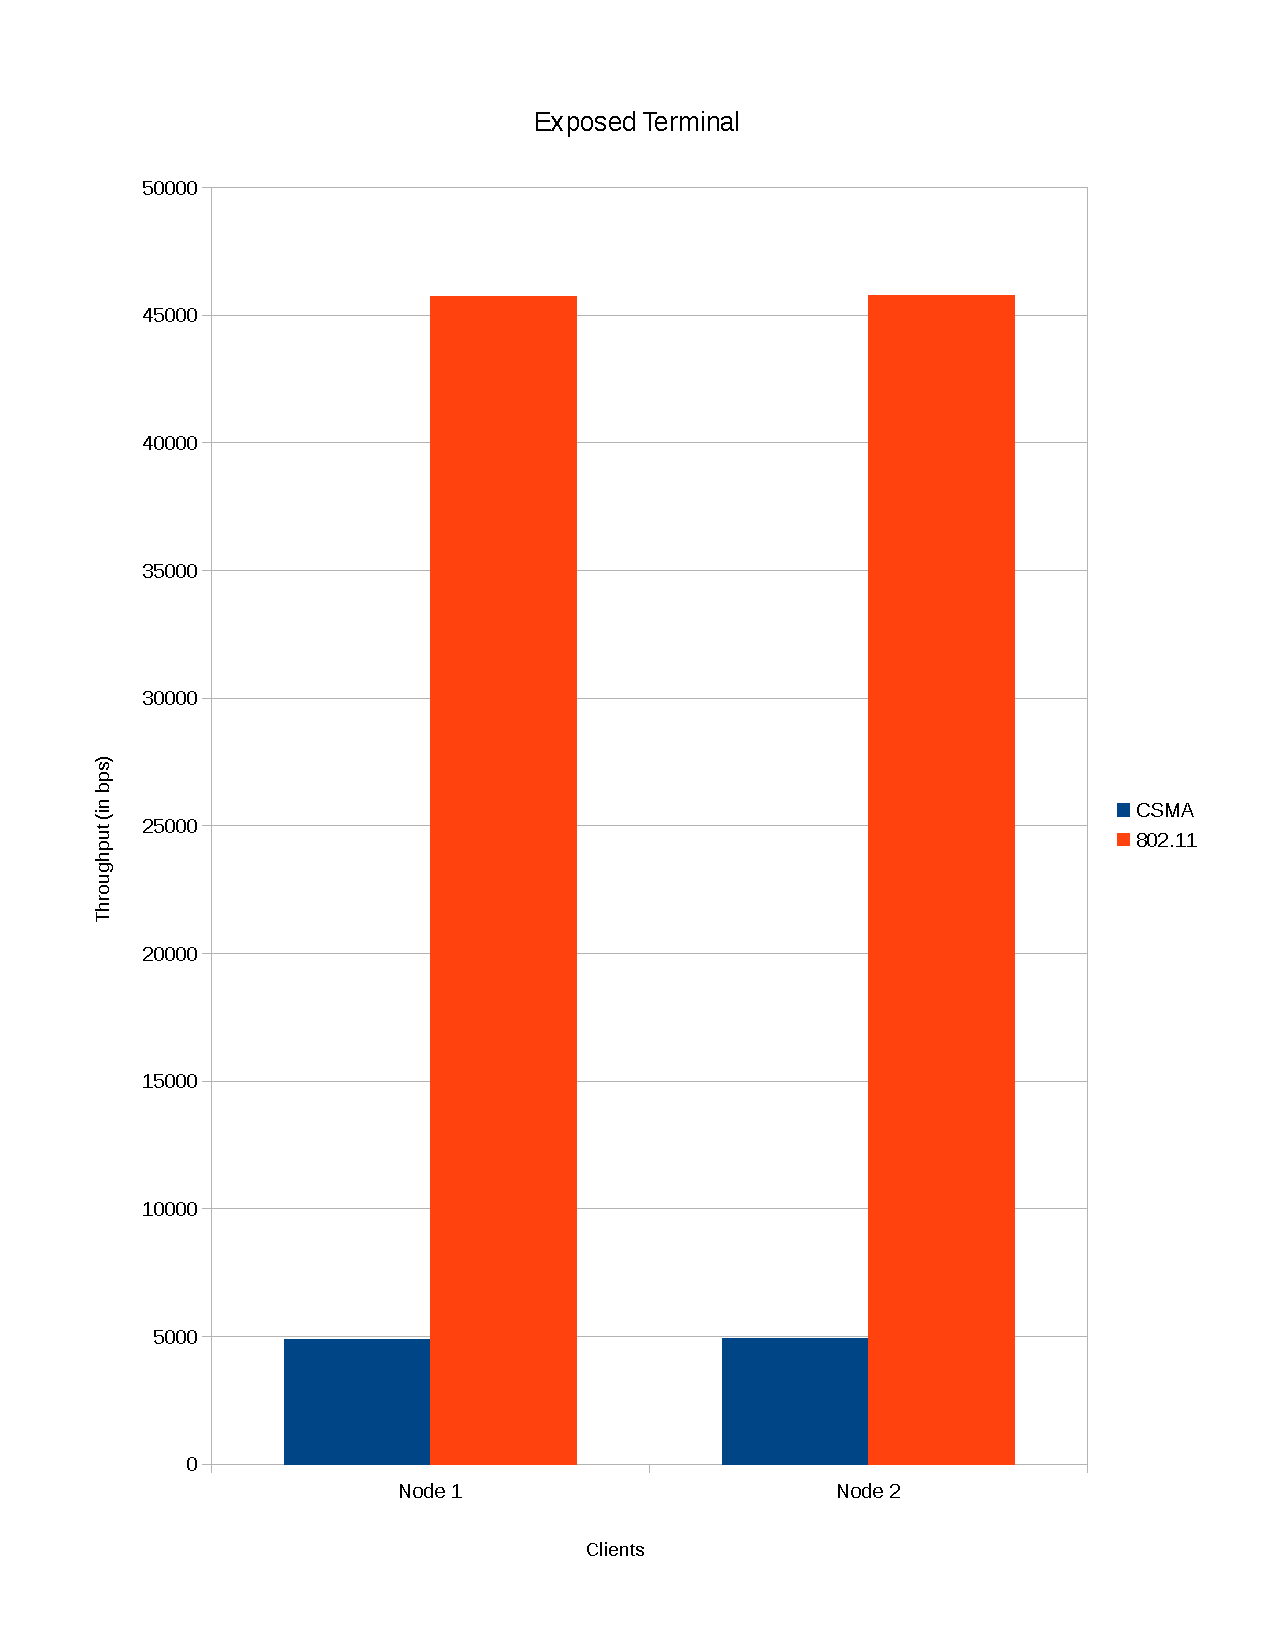
\includegraphics[width=0.35\textwidth, scale=0.5]{figures/exposed_thrput.pdf}
  \caption{Change in the throughput when the MAC protocol is changed from CSMA to 802.11}
  \label{fig:overhead}
\end{figure}

\subsection{Sample Use Cases}

\subsubsection{Hidden Terminal}
The Hidden terminal problem occurs in wireless networks when a node is visible from a particular destination node, but is not visible from other nodes that are communicating with the destination node. Since the transmitting nodes are out of range of one another, CSMA cannot detect a transmission and collisions occur as a result. IEEE 802.11 solves this problem with the help of the RTS/CTS mechanism. Since all trasmitting nodes are within communication range of the destination, they can hear the CTS destined to a particular transmitter. This ensures that only one transmitter communicates with the node. 

We start the simulation with all nodes running CSMA as the MAC protocol. The test controller then issues the \emph{SWTICH-MAC} command with the appropriate MAC protocol (WIFI-PROTO) and forwards the request to all the nodes in the simulation. On each node, we first wait for the in-flight packets to be serviced and the state of the radio to become idle, and then initialize the MAC protocol to 802.11. Waiting for the radios to become idle is an approximation of the 4-way handshake described earlier. We also ensure that the simulation statistics of the nodes under both the original and the changed MAC protocols are saved in glomo.stat. As it is evident from the plots, 802.11 out performs CSMA both in throughput and the number of packets successfully received.

\subsubsection{Exposed Terminal}
The Exposed Terminal problem occurs in wireless networks when a node is not allowed to send packets to other nodes because of the presence of a transmitting node within its radio range, even though the receivers of the two nodes are out of range of each other. In CSMA, a node that wants to send packets performs carrier sense and after sensing the neighbours transmission, decides not to transmit as it would result in interfernce. IEEE 802.11, on the other hand, solves this problem with the help of the RTS/CTS mechansim. A node can identify itself as an exposed node if it hears an RTS from a neighbouringnode, but does not hear a corresponding CTS. It can then transmit to its intended receivers. 
Similar to the \emph{Hidden terminal} use case, we start the simulation with all the nodes running CSMA and then, the test controller issues the \emph{SWTICH-MAC} command with the appropriate MAC protocol (WIFI-PROTO) and forwards the request to all the nodes in the simulation. On each node, we wait for the in-flight packets to be serviced and the state of the radio to become idle, and then initialize the MAC protocol to 802.11, which is the approximation for the 4-way handshake. We also ensure that the simulation statistics of the nodes under both MAC protocols are saved in glomo.stat. As it is evident from the plots, 802.11 out performs CSMA both in throughput and the number of packets successfully received.  

%\input{experiment}
% \input{discussion}
%\section{Applications}

\subsection{Frequency Hopping}
Frequency hopping is a technique of transmitting radio signals by spreading the signal over a sequence of changing frequencies. It has tremendous application in military as it is used against jamming and for protecting against unauthorized eavesdropping. For implementation, the receiver of the signal must be aware of the sequence of frequencies so that it can tune into the appropriate channel. This requires synchronization between the transmitter and the receiver. In \crossflow, we implement this application easily as only the controller needs to be aware about the predetermined sequence. This sequence can even be dynamic according to the channel conditions and policies. The controller simply issues \emph{GNU-CONFIG-FREQ} command with desired frequency and pushes this configuration to the device. The \texttt{ofsoftswitch} receives this command and forwards it to the GNU Radio domain. The centralized \texttt{\crossflow Hub} inside the GNU Radio domain processes this request and issues appropriate commands to the  USRP Controller, which ultimately signals the USRP block to tune into the requested frequency. Figure~\ref{fig:freq} shows the experimental results where the sequence of changing frequencies is 910, 915 and 920 MHz and is changed every 5 seconds with BPSK fixed modulation scheme.   

\subsection{Adaptive Modulation}
Adpative Modulation is a technique where the modulation is changed according to the conditions of the channel. There are various estimators which are used for obtaining channel quality. These can be Signal-to-noise ratio (SNR), Bit error rate (BER) and other environment specific estimators. For illustration, we assume a fixed sequence for changing the modulation schemes every 5 seconds. Similar to the \emph{frequency hopping} application, the controller issues the \emph{GNU-CONFIG-MOD} command with the appropriate modulation scheme like BPSK, QPSK etc and forwards the request to the device. The request ultimately reaches the MOD controller, which is a multiplexer block that selects the requested modulation scheme. Figure~\ref{fig:mod} shows the results for changing the modulation scheme between BPSK, QPSK and 8PSK every 5 seconds, keeping a fixed carrier frequency of 910 MHz.   


\section{Conclusion and Future Work}
\label{sec:conclusion}
In this paper, we presented a framework for programming a network of software defined radios using  software defined networking (SDN) principles. The framework we propose allows adaptive, flexible, and real-time (re)configuration of software defined radio interfaces from a network controller application. It streamlines the development of network applications by hiding the low level  internal details of the signal processing pipeline. In order to validate our approach, we also provide three proof-of-concept applications: \emph{frequency hopping}, \emph{adaptive modulation} and \emph{cognitive radio}. This shows that our design is viable and can be extended to introduce new capabilities.

One of the challenges that we need to consider is in-band control of the radio devices. Currently we implemented our design using an out-of-band wired control channel. The \crossflow framework can easily be extended to enable in-band control of devices and it will be our next design goal. Another area of focus is the latency between controller and SDR framework. The issue can be mitigated, by the introduction of distributed control module in SDR. The distributed control module will allow devices to take local decisions while the centralized controller is responsible for introducing policies and global management, thereby ensuring reduced latency.
The \crossflow framework can also be extended to allow controller to create other abstract radio blocks and manipulate inter-connections between those radio blocks. It requires design of new APIs on switch agent and can be implemented by combining the methodology provided by GNU Radio. In GNU radio, each block has an input and output port and the application needs to specify the connecting ports in order to connect the blocks. Only ports which are similar, i.e, ports which operate on same types of data(message or stream), can connect to each other. The data type supported by a block can be obtained by sending capability messages. The decision whether two ports are compatible can be left to the application. 

%\input{acks}

\bibliographystyle{plain}
\bibliography{references}

\end{document}
